\let\negmedspace\undefined
\let\negthickspace\undefined
\documentclass[journal]{IEEEtran}
\usepackage[a5paper, margin=10mm, onecolumn]{geometry}
\usepackage{lmodern} % Ensure lmodern is loaded for pdflatex
\usepackage{tfrupee} % Include tfrupee package

\setlength{\headheight}{1cm} % Set the height of the header box
\setlength{\headsep}{0mm}     % Set the distance between the header box and the top of the text

\usepackage{gvv-book}
\usepackage{gvv}
\usepackage{cite}
\usepackage{amsmath,amssymb,amsfonts,amsthm}
\usepackage{algorithmic}
\usepackage{graphicx}
\graphicspath{{./figs/}}
\usepackage{textcomp}
\usepackage{xcolor}
\usepackage{txfonts}
\usepackage{listings}
\usepackage{enumitem}
\usepackage{mathtools}
\usepackage{gensymb}
\usepackage{comment}
\usepackage[breaklinks=true]{hyperref}
\usepackage{tkz-euclide} 
\usepackage{listings}
\usepackage{gvv}                                        
\def\inputGnumericTable{}                                 
\usepackage[latin1]{inputenc}                                
\usepackage{color}                                            
\usepackage{array}                                            
\usepackage{longtable}                                       
\usepackage{calc}                                             
\usepackage{multirow}                                         
\usepackage{hhline}                                           
\usepackage{ifthen}                                           
\usepackage{lscape}
\usepackage{circuitikz}
\tikzstyle{block} = [rectangle, draw, fill=blue!20, 
text width=4em, text centered, rounded corners, minimum height=3em]
\tikzstyle{sum} = [draw, fill=blue!10, circle, minimum size=1cm, node distance=1.5cm]
\tikzstyle{input} = [coordinate]
\tikzstyle{output} = [coordinate]
\begin{document}
\bibliographystyle{IEEEtran}
\vspace{3cm}
\title{4.11.27}
\author{EE25BTECH11050-Hema Havil}
	\maketitle
	% \newpage
	% \bigskip
	{\let\newpage\relax\maketitle}
	
	\renewcommand{\thefigure}{\theenumi}
	\renewcommand{\thetable}{\theenumi}
	\setlength{\intextsep}{12pt} % Space between text and floats
	
	\numberwithin{equation}{enumi}
	\numberwithin{figure}{enumi}
	\renewcommand{\thetable}{\theenumi}
	
	\textbf{Question}:\\
    
         Find the coordinates of the point where the line through $(4,-3,-4)$ and $(3,-2,2)$ crosses the plane $2x+y+z=6$
         
         \solution \\
         Let the given points be P(4,-3,-4) and Q(3,-2,2) then the direction vector along pq be d, 
         \begin{align}
             \vec{d}=\vec{Q}-\vec{P}=\myvec{3\\-2\\2}-\myvec{4\\-3\\-4}=\myvec{-1\\1\\6}
         \end{align}
         equation of line passing through P,Q be
         \begin{align}
             r(t)=r_0+td
         \end{align}
         where t is a parameter
         \begin{align}
             \vec{r(t)}=\myvec{4\\-3\\-4}+t\myvec{-1\\1\\6}
         \end{align}
         Let the given plane equation be 
         \begin{align}
             \vec{n}^T\vec{x}=c 
         \end{align}
         where, 
         \begin{align}
             \vec{n}=\myvec{2\\1\\1}\\
             c=6
         \end{align}
         Consider a point with parameter $t_1$ which is the intersection point then, it satisfies line equation and plane equation 
         \begin{align}
             \vec{r(t_1)}=\myvec{4\\-3\\-4}+t_1\myvec{-1\\1\\6}
         \end{align}
         Substitute this point in the plane equation 
         \begin{align}
             \vec{n}^T\vec{r_{t_1}}=c
         \end{align}
         \begin{align}
             \myvec{2\;1\;1}\brak{\myvec{4\\-3\\-4}+t_1\myvec{-1\\1\\6}}=6
         \end{align}
         \begin{align}
             1+t_1\brak{5}=6
         \end{align}
         \begin{align}
             5t_1=5
         \end{align}
         \begin{align}
             t_1=1
         \end{align}
         then the intersection point be,
         \begin{align}
             \vec{r_{t_1}}=\myvec{4\\-3\\-4}+\myvec{-1\\1\\6}
         \end{align}
         \begin{align}
             \vec{r_{t_1}}=\myvec{3\\-2\\2}
         \end{align}
         \begin{figure}[h]
             \centering
             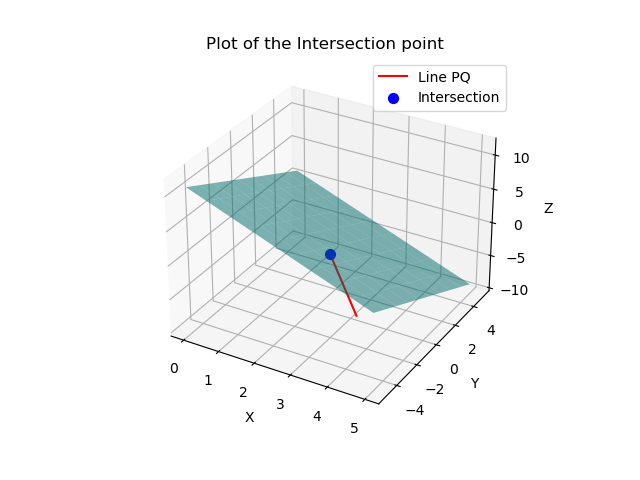
\includegraphics[width=0.7\columnwidth]{figs/fig1.png}
             \caption{Plot of the Intersection point}
             \label{fig1}
         \end{figure}
         
\end{document}

